\documentclass[11pt]{standalone}

\usepackage{pgfplots}
\usetikzlibrary{hobby}
\pgfplotsset{compat=newest}

\begin{document}
	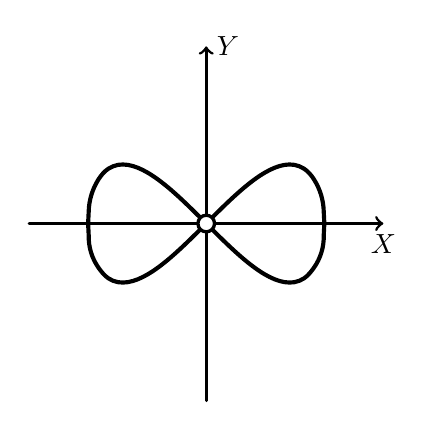
\begin{tikzpicture}[line cap=round, line join=round]
	\draw[->, line width=1] (-2.25,0) -- (2.25, 0) node[below] {$X$};
	\draw[->, line width=1] (0,-2.25) -- (0,2.25) node[right] {$Y$};
	\draw[line width=1.5] (-1.5,0) -- plot[domain=-0.995:0.995,variable=\x,% orange,
	 line width=1.5, quick hobby] (1.5*\x, {1.5*\x *sqrt(1-\x*\x)}) -- (1.5,0) -- plot[domain=-0.995:0.995,variable=\x,quick hobby] (-1.5*\x, {1.5*\x *sqrt(1-\x*\x)}) -- cycle;
	\draw[%orange, 
	fill=white, line width=1.2pt] (0,0) circle (3pt);
	\end{tikzpicture}
\end{document}